% -O2 with debug level on (20 runs per case)
% Case1: 
% Vector length (N)     = 52
% Total ticks           = 219
% Average ticks         = 10
% Result f(x)           = 170105728.000000
% Program size: 75 KBytes program size (code + initialized data).
%               302 KBytes free for stack + heap.

% Case2: 
% Vector length (N)     = 2041
% Total ticks           = 8712
% Average ticks         = 435
% Result f(x)           = 6627435008.000000
% Program size: 82 KBytes program size (code + initialized data).
%               294 KBytes free for stack + heap.

% Case3:
% Vector length (N)     = 65281
% Total ticks           = 287628
% Average ticks         = 14381
% Result f(x)           = 211932430336.000000
% Program size: 329 KBytes program size (code + initialized data).
%               47 KBytes free for stack + heap.

% Case4:
% Vector length (N)     = 2323
% Total ticks           = 10114
% Average ticks         = 505
% Result f(x)           = 7668609536.000000
% Program size: 84 KBytes program size (code + initialized data).
%               293 KBytes free for stack + heap.


% Python results:
% Case 1: N=52, f(x)=1.7010572800e+08
% Case 2: N=2041, f(x)=6.6274365440e+09
% Case 3: N=65281, f(x)=2.1193741107e+11
% Case 4: N=2323, f(x)=7.4612725760e+09


\begin{figure}[H]
    \centering
    \fbox{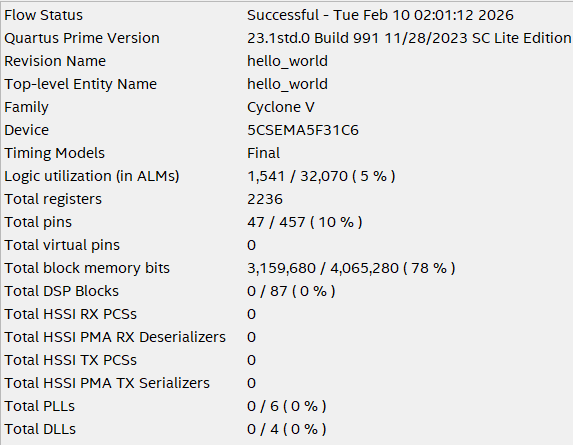
\includegraphics[width=0.95\linewidth]{Images/task3_resource_util.png}}
    \caption{Task 3 FPGA resource utilization snapshot.}
    \label{fig:task3_resource_placeholder}
\end{figure}
